\section{Parallel Strategy and Performance}
\label{sec.parallel}

\subsection{Parallel Strategy}

% GB to work on this
%  - expand to include better description
%  - include load balancing options

When \enzo\ is run on a distrubuted platform, some of the data is
replicated to all processors, while some remains on a single processor.
A description of the entire hierarchy (the position and size of each grid, as well
some other meta data) is stored on each processor.  This enables each
grid to know what grids are near it in the hierarchy, regardless of
where the data is.  The actual Baryon data (density, velocity, energy,
and any chemistry data) and particle data are stored on only one
processor.  Storing the entire hierarchy on all processor does create
some overhead, but in practice this is not an issue until one reaches
the extremely large scale.
  The code handles load balancing 
on a level-by-level basis such that the workload on each level is 
distributed as uniformly as possible across all processors.  Spatial locality of 
grids is not forced during message passing, for maximum flexibility (though not
necessarily maximum efficiency).  
The MPI message passing library\footnote{http://www-unix.mcs.anl.gov/mpi/}
 is used to transfer data between processors.
 
 


%old text
%Every processor 
%keeps a description of the entire grid hierarchy at all times, so that 
%each processor knows where all grids are.  However, baryon and particle 
%data for a given grid only exists on a single processor.  See 
%Figure~\ref{fig.2.amrhierarchy} for a schematic example of this.  



\begin{figure}
\begin{center}
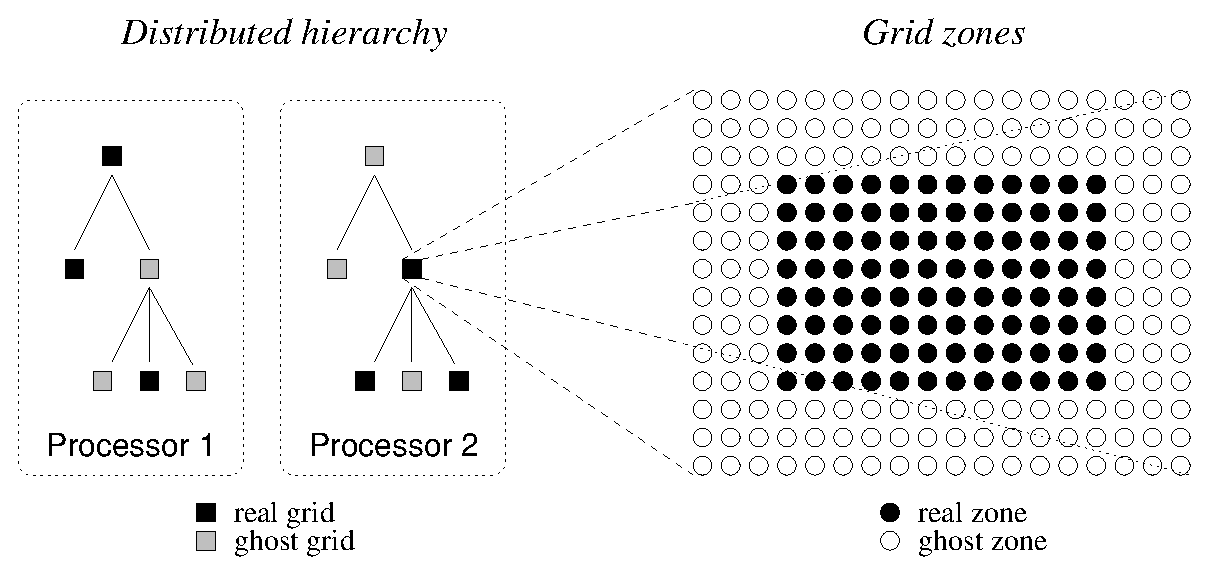
\includegraphics[width=0.4\textwidth]{figures/amr_hierarchy.eps}
\end{center}
\caption{\emph{Left:}  Example of a simple, distributed AMR hierarchy showing real and ghost grids.
\emph{Right:}  Example 2D \enzo\ grid showing real and ghost zones, as 
needed for the PPM hydro stencil. }
\label{fig:amr_hierarchy}
\end{figure}



% ----------------------------------

\subsection{Performance}
\label{sec.performance}

\subsubsection{Performance model \red{(Greg)}}

% Maybe include Greg's text on general scaling arguments

\subsubsection{Performance Measurement \& Instrumentation \red{(Sam)}}

Because of the wide variety of simulations, methods, and uses of Enzo,
it is difficult to define exactly which routines are most costly
during a given simulation.  As such, we have designed a lightweight
registering system that has been implemented for the most commonly
used routines (such as the hydrodynamic and gravity solvers) as well
as refinement level timers that measure the (exclusive) time spent on
each level.  Beyond this minimal set of routines, we have designed a
simple way for the user to modify the source by adding
\texttt{TIMER\_START(``Your Routine Name'')} and
\texttt{TIMER\_END(``Your Routine Name'')}.  These timers are
automatically registered in a
std::map\footnote{http://www.cplusplus.com/reference/map/map/}.  These
timers are created and managed individually on each processor in an
asynchronous fashion.

At each complete EvolveHierarchy (or less often if specified), each timer is
then communicated to the root processor where it calculates the mean, standard
deviation, minimum, and maximum for each of the timers across all processors. 
For level timers, there are also attributes such as the number of cell updates,
the current number of grids, and the average cells/s/MPI process.  This
information is then output to a ``performance.out'' logfile.  This provides a 
simplified interface to the user that can be used to diagnose performance 
issues as well as estimate a given problem type's scalability.  In addition to 
the logfile, we have developed a plotting interface for quickly producing 
figures that process the data from the logfile.  These capabilities are 
described in the online documentation, along with a further discussion of the 
performance measurement implementation.

\subsubsection{Unigrid scaling}
\label{sec:weak_scaling}

\begin{figure}
\begin{center}
\includegraphics[width=0.6\textwidth]{figures/enzo_unigrid_weak_scaling.eps}
\caption{\enzo\ weak scaling performance for a set of Lyman alpha
forest cosmology simulations with constant comoving spatial resolution
per grid cell, showing cell updates per second per computational core
plotted as a function of the number of root grid tiles of dimension
$128^3$ (R) in each dimension.  The number of MPI tasks is N$ = R^3$,
so R$ = 16$ on this plot corresponds to a $2048^3$ computational mesh
running on 4,096 MPI tasks.  This plot goes from R$ = 2$ (8 MPI tasks)
to R$ = 24$ (13,824 MPI tasks) on two supercomputers -- NICS Kraken
and ORNL Jaguar when they were Cray XT4 systems -- and using 1, 2 or 4
MPI processes per node, where each compute node contained a single
quad-core AMD Opteron CPU having a speed of 2.1 GHz on Jaguar and 2.3
GHz on Kraken.}
\label{fig.uniscale}
\end{center}
\end{figure}

It is advantageous to use \enzo\ in its ``unigrid'' (i.e.,
non-adaptive mesh) mode for a variety of problems, including
non-gravitating turbulence
\citep[e.g.,][]{2002ApJ...569L.127K,Kritsuk04}, the Lyman-alpha forest
\citep{2005MNRAS.361...70J,2009MNRAS.399.1934P}, or feedback of
metal-enriched gas from galaxies into the intergalactic medium
\citep{2004ApJ...601L.115N,2011ApJ...731....6S}.  Achieving good
scaling of the code in unigrid mode is relatively straightforward --
upon initialization, unigrid simulations are decomposed such that each
MPI process has a roughly equal subvolume (and thus number of grid
cells), meaning that work is evenly distributed.  Communication
patterns for both the gravity solve (which uses a fast Fourier
transform) and the fluid solves (which transfer boundary information
between subvolumes) are predictable and straightforward, and
rebuilding of the grid hierarchy does not take place, removing a
substantial global operation and a great deal of communication.

Figure~\ref{fig.uniscale} shows \enzo\ weak scaling results for a
sequence of scaled unigrid Lyman alpha forest calculations. These
calculations include dark matter dynamics, hydrodynamics using the
piecewise parabolic method, six-species non-equilibrium chemistry and
radiative cooling, and a uniform metagalactic ultraviolet background.
In this sequence of test calculations, we perform a weak scaling test
on up to 13,824 MPI tasks on the NICS Kraken XT4 and ORNL Jaguar XT4
supercomputers\footnote{These simulations were performed in 2008,
prior to conversion of both machines to the current-generation
systems}.  In this test, each MPI task was given a $128^3$ root grid
tile (i.e., $128^3$ grid cells containing baryon quantities) and,
initially, approximately $128^3$ dark matter particles.  The number of
grid cells was constant throughout the calculation; the number of dark
matter particles varies as they are moved from subvolume to subvolume
as structure evolves.  The grid resolution was kept at a constant
comoving size of $\simeq 40$~kpc/h, and as the core count was
increased, so was the simulation volume.  On each machine, a compute
node contained a single AMD Opteron quad-core chip (2.1 Ghz on Jaguar;
2.3 Ghz on Kraken) with 2 GB/memory per core (8 GB/total per node).
Both machines used the SeaStar2 interconnect.  In the scaling study,
calculations were run with 1, 2 or 4 MPI tasks per node.  The figure
shows cell updates per second per MPI process; perfect scaling would
be a horizontal line.

As can be seen in Figure~\ref{fig.uniscale}, the unigrid weak scaling
performance of the code is extremely good for this problem, with only
a 20\% decrease in cell updates/second/task as the code is scaled from
8 to 4,096 MPI tasks, and a 40\% decrease in performance overall going
from 8 to 13,824 (or $24^3$) MPI tasks.  We speculate that this
decrease is likely to be partially due to global MPI communications
used to, e.g., calculate the overall timestep of the simulation, and
also likely due to load imbalances due to increasing cosmological
power (and thus an increasingly uneven distribution of dark matter
particles between MPI tasks at late times) as the simulation volume
grows.  We also observe that a systematic difference in speed can be
seen between the two machines, which can be attributed primarily to
the slightly faster CPUs on Kraken (2.3 Ghz, vs. 2.1 Ghz on Jaguar).
The difference in speed when using different numbers of MPI tasks per
node can be attributed primarily due to differences in competing usage
of shared cache on the quad-core chips used on this machine.

Broadly, excellent scaling in \enzo's unigrid mode is seen for a
variety of problems as long as each compute core is given an adequate
amount of work to do.  For cosmological simulations, this seems to be
roughly $128^3$ cells per core.  If fewer cells per core are used, the
CPU is essentially data-starved, and poor scaling is observed due to
computing units being idle while waiting for information to be
communicated from other processes (for, e.g., boundary information or
gravity solves).  Substantially larger cell counts per core would in
principle help scaling by reducing the amount of inter-process
communication needed, but larger cell counts are typically impractical
on most machines due to memory limits.

As a final point, we observe that scaling at larger core counts has
been measured, but only with an experimental hybrid-parallel (MPI +
OpenMP) version of \enzo.  Using this version, scaling comparable to
that shown in Figure~\ref{fig.uniscale} was seen on up to 98,304 cores
on the NICS Kraken XT5 (an upgraded version of the XT4 machine used
for the scaling study shown in the figure), using 2-8 OpenMP threads
per MPI process.  Hybrid parallelism has the potential to
substantially improve scaling by reducing the amount of communication
per grid tile (as described in the previous paragraph); however, the
optimal ratio of OpenMP threads per MPI task seems to vary
substantially between computational platforms and astrophysical
problems/required \enzo\ physics modules, and thus we hesitate to
provide strict guidelines here.

\subsubsection{AMR scaling}

\begin{figure}
\begin{center}
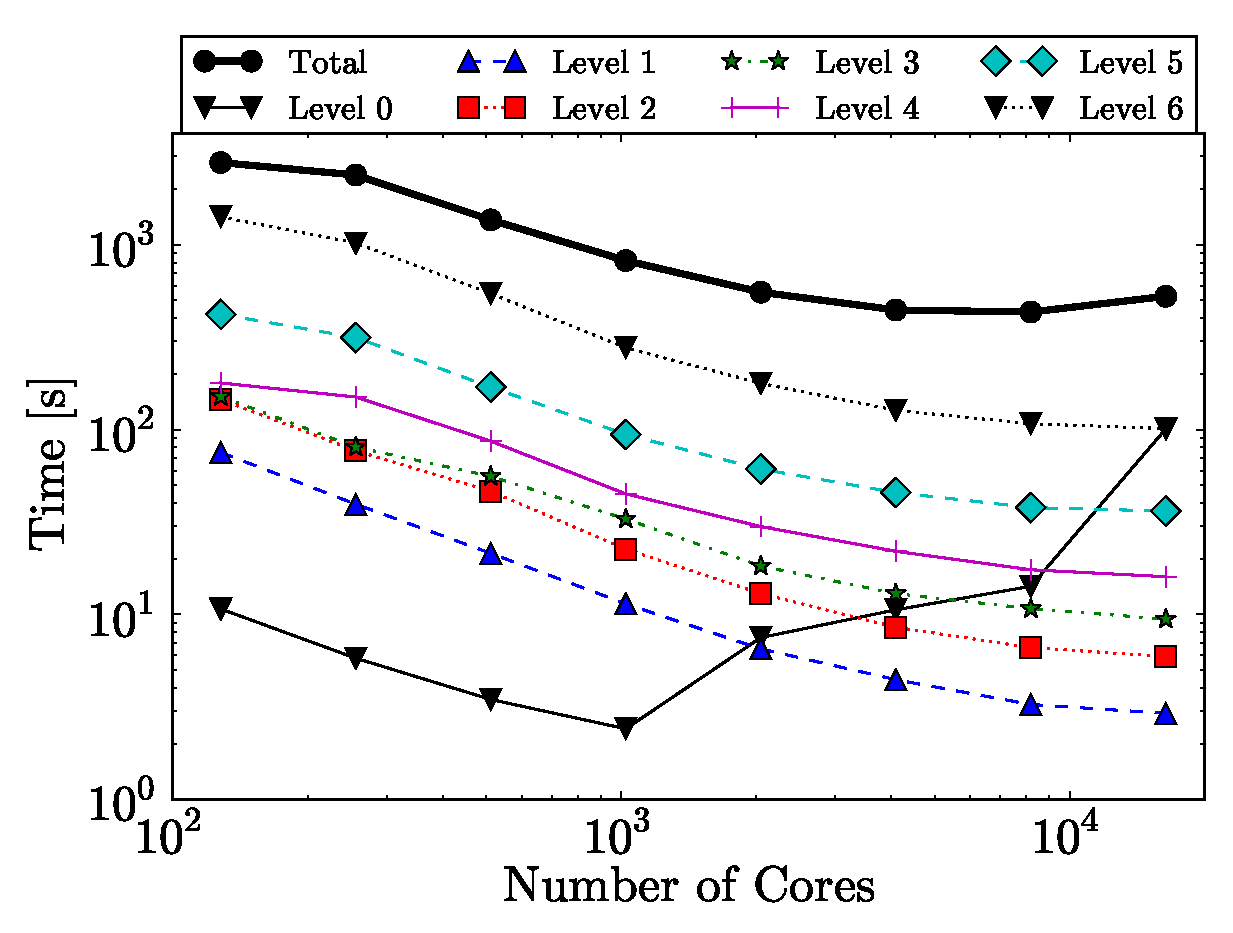
\includegraphics[width=0.48\textwidth]{figures/strong_scaling_levels.eps}
\hfill
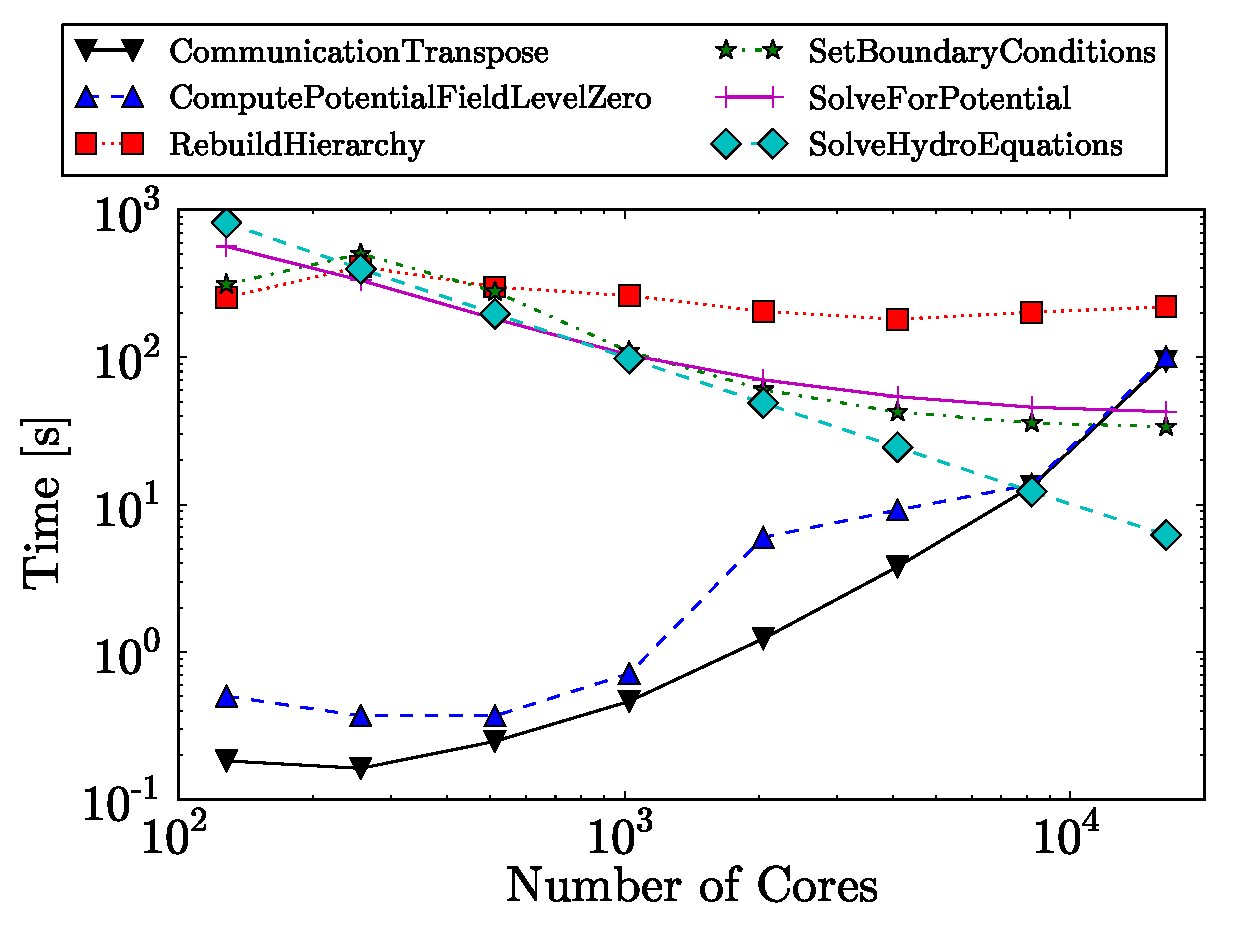
\includegraphics[width=0.48\textwidth]{figures/strong_scaling_routines.eps}
\end{center}
\caption{\emph{Left:} Strong scaling test of a 512$^3$ AMR
  cosmological calculation.  The root grid scaling is not
  representative of the true strong scaling of Enzo because the root
  grid tiles are not repartitioned when a simulation is restarted with
  additional cores.  The weak scaling test in Figure
  \ref{fig.uniscale} is more representative of the scaling on the root
  level.  The performance in the refined levels show good strong
  scaling up to 2,048 cores.  \emph{Right:} Time spent in
  representative major routines in the same AMR calculation.}
\label{fig:strong_scaling}
\end{figure}

Many astrophysical problems, such as cosmological galaxy formation
\citep{}, high-resolution disk galaxy simulations \citep{},
high-redshift \citep{} and present-day star formation \citep{},
involve multi-scale physics that span several orders of magnitude in
both space and time.  In these situations, using Enzo in its adaptive
mesh refinement mode is beneficial.  Because the adaptive grid
hierarchy is dynamic and not static, grid boundaries and, thus,
communication patterns can be unpredictable, hindering good strong
scaling at high core counts.

Figure \ref{fig:strong_scaling} shows strong scaling results from a
single 50 Mpc/h cosmology simulation run on $N_{\rm core}$ compute
cores, ranging from 128 to 16,384 at power-of-two intervals.  It was
run on the NICS Kraken XT5 supercomputer that has two AMD Opteron
hexa-core processors with 16 GB of memory per compute node.  The
simulations that utilized 128, 256, and 512 cores were executed on 128
nodes because of the memory requirements.  The higher core count jobs
were run with 8 cores per node.  This simulation would not run with 12
cores per node because of the memory overhead associated with the grid
hierarchy being duplicated on each MPI process.  However, this
overhead is greatly diminished if a hybrid-parallel (MPI + OpenMP)
approach is used.

This simulation includes dark matter dynamics, hydrodynamics using the
piecewise parabolic method, six-species non-equilibrium chemistry and
radiative cooling, and a uniform metagalactic ultraviolet background.
The simulation uses the space-filling curve method for load balancing
the AMR grids.  It has a $512^3$ root grid that is divided into 512
tiles, and 6 additional AMR levels are used.  We perform these scaling
tests when the simulation reaches $z=4$.  The results shown in Figure
\ref{fig:strong_scaling} come from a single root-level timestep
$\Delta t = 2.1\, \textrm{Myr}$.  At this time, there are $3.04 \times
10^5$ AMR grids, $9.03 \times 10^8$ ($\sim 967^3$) computational
cells, and $1.34 \times 10^8$ dark matter particles in total.  The
breakdown of the number of AMR grids, cells, timesteps, and number of
cell updates on each level is shown in Table \ref{tab:amr_scale}.

%%%%%%%%%%%%%%%%%%%%%%%%%%%%%%%%%%%%%%%%%%%%%%%%%%%%%%%%%%%%%%%%%%%%%%%%
\begin{table*}
  \begin{center}
  \caption{Strong scaling test computational details}
  \begin{tabular*}{0.9\textwidth}{@{\extracolsep{\fill}}c c c c c}
    \tableline\tableline
    {Level} & {$N_{\rm grid}$} & {$N_{\rm cells}$} & {$N_{\rm up}$} &
    {$N_{\rm timesteps}$}\\
    \tableline
    0 & 512 & $1.34 \times 10^8$ & $1.34 \times 10^8$ & 1\\
    1 & 61,868 & $4.01 \times 10^8$ & $4.01 \times 10^8$ & 1\\
    2 & 91,182 & $1.99 \times 10^8$ & $5.96 \times 10^8$ & 3\\
    3 & 59,932 & $7.62 \times 10^7$ & $5.34 \times 10^8$ & 7\\
    4 & 40,700 & $3.32 \times 10^7$ & $5.65 \times 10^8$ & 17\\
    5 & 28,346 & $2.76 \times 10^7$ & $1.36 \times 10^9$ & 49\\
    6 & 19,771 & $2.80 \times 10^7$ & $5.25 \times 10^9$ & 187\\
    \tableline
    Total & 302,311 & $9.03 \times 10^8$ & $8.83 \times 10^9$ & --\\
  \end{tabular*}
  \parbox[t]{0.9\textwidth}{\textbf{Note.} --- Data shown at $z=4$ for
    a root grid timestep of 2.1~Myr.  Col. (1): AMR Level. Col. (2):
    Number of grids. Col. (3): Number of computational
    cells. Col. (4): Number of cell updates. Col. (5): Number of
    timesteps.}
  \label{tab:amr_scale}
  \end{center}
\end{table*}

%%%%%%%%%%%%%%%%%%%%%%%%%%%%%%%%%%%%%%%%%%%%%%%%%%%%%%%%%%%%%%%%%%%%%%%%

The left panel in Figure \ref{fig:strong_scaling} shows the
computational and communication time spent on each level.  In the AMR
levels, there exists good strong scaling up to 2,048 cores, and
marginal speed-ups are found at 4,096 cores.  On the root-grid level,
there exists good scaling up to 1,024 cores, but the performance
dramatically decreases at higher core counts.  This occurs because the
root grid is not re-partitioned into $N_{\rm core}$ tiles when the
simulation is restarted with a different core count.  This feature can
be easily implemented and is planned in the next major release of
Enzo, where scaling results would be similar to the weak scaling shown
in \S\ref{sec:weak_scaling}.  The right panel in Figure
\ref{fig:strong_scaling} shows the time spent in some representative
major routines in Enzo.  The local physics routines, for example
\texttt{SolveHydroEquations}, exhibit perfect strong scaling because
they involve no communication.  By investigating the scaling behavior
in each routine, it is clear that the communication in the
\texttt{SetBoundaryConditions}, \texttt{SolveForPotential} (multi-grid
solver in AMR levels), and \texttt{RebuildHierarchy} are responsible
for the lack of strong scaling at $N_{\rm core} \ga$~4,096 in this
particular simulation.  The transpose of the root grid tiles are
responsible for the performance decrease because it is not optimized
for situations where the number of tiles is greater than the number of
MPI processes.  These results are directly applicable to simulations
with similar computational demands.  In simulations with less
computational cells, strong scaling will cease at a smaller core count
because the CPUs will become data-starved faster, and the opposite
occurs with larger simulations.

%%% Local Variables: 
%%% mode: latex
%%% TeX-master: "ms"
%%% End: 
